%% CHAPTER HEADER /////////////////////////////////////////////////////////////////////////////////////
\chapter[Methodology]{Methodology}
\label{ch4}

%% CHAPTER INTRODUCTION ///////////////////////////////////////////////////////////////////////////////
In this chapter, several DL methodologies were presented in order to detect and localise delamination in composite laminates based on non-contact ultrasonic wavefield imaging that can provide precise details about the health status of the investigated specimen.
Accordingly, a large synthetic dataset was generated representing the full wavefield of the Lamb waves propagating in a CFRP plate and their interaction with discontinuities such as the delamination and the plate edges, acquired by SLDV from the bottom surface of the plate.
The acquisition process of the synthetic dataset is explained in details in the section~\ref{sec41}.

The deep learning models were trained using a supervised scheme. 
Hence, it uses a training set to train the developed models to predict the desired output.
The developed methods are end-to-end approaches, in which the whole unprocessed training dataset is fed into the model.
Hence, it will learn by itself to identify distinct patterns and detect damage.
In section~\ref{sec42}, a fully connected CNN classifier model for detecting and localising delamination is presented in details.
In section~\ref{sec43}, I present five FCN models for delamination identification. 
Further, the developed models were trained using the RMS images in which the developed models are performing pixel-wise image segmentation.
In section~\ref{sec44}, a deep learning model for delamination identification utilising the animation of full wavefield is presented.

As mentioned earlier, ultrasonic wavefield imaging with SLDV can provide detailed information on the health status of an inspected structure.
However, high spatial resolution, which is frequently required for precise damage size estimation, typically demands a prolonged scanning time.
In section~\ref{sec45}, I present a DL model for image super-resolution reconstruction in which the full wavefields of Lamb waves are recovered from low-resolution wavefields acquired with a reduced number of measuring points into high-resolution wavefields.
Accordingly, this can allow for a precise recovery of propagating waves and their interactions with discontinuities such as delaminations and boundaries of the plate.
Consequently, this process will speed up the acquisition of data.
Furthermore, the reconstructed full wavefield can be used in damage imaging. 


All developed models were implemented and trained with the Keras API~\cite{chollet2015keras} running on top of TensorFlow~\cite{Abadi2016}.
The NVIDIA GeForce RTX 2070 with \(8\) GBs of memory was utilised to train the CNN classification models.
Furthermore, the NVIDIA Tesla V100 GPU with \(32\) GBs of memory was utilised to train the FCN models, the AE-ConvLSTM model, and the DLSR model.
%% INCLUDE SECTIONS ///////////////////////////////////////////////////////////////////////////////////

%% SECTION HEADER /////////////////////////////////////////////////////////////////////////////////////
\section{Synthetic data acquisition}
\label{sec41}
%%%%%%%%%%%%%%%%%%%%%%%%%%%%%%%%%%%%%%%%%%%%%%%%%%%%%
The crucial part in our work was in synthetically generating a dataset of a full wavefield of propagating of Lamb waves in a plate made of CFRP.
In which we
In this work, we have generated a large dataset of \(475\) cases of a full wavefield of propagating Lamb waves in a plate made of carbon fibre-reinforced plastic (CFRP).
The in-house code of the time-domain spectral element method was used for simulation of Lamb wave interaction with delamination~\cite{Kudela2020}.
It should be added that despite the utilisation of the parallel code of the spectral element method which was run on the Tesla K20X GPU card, the computation of the dataset (consisting of 475 cases) took about 3 months.
For each case, single delamination was modelled by using the method of splitting nodes between appropriate spectral elements. 
It was assumed that the composite laminate is made of eight layers of a total thickness of 3.9 mm.
The delamination was modelled between the third and fourth layer (see Fig.~\ref{fig:plate_setup} for details).
It should be noted that Fig.~\ref{fig:plate_setup} shows an exaggerated cross-section through the delamination. 
Zero-volume delamination was assumed in the model. 
Delamination spatial location was selected randomly so that the interaction of guided waves with delamination is different for each case.
It includes cases when delamination is located at the edge of the plate which is the most difficult to identify by signal processing methods.
Additionally, the size of the delamination of elliptic shape was randomly simulated by selecting the size of ellipse minor and major axis.
Also, the angle between the delamination major axis and the horizontal axis was randomly selected.
In summary the following random factors were simulated in each case:
\begin{itemize}
	\item delamination geometrical size	(ellipse minor and major axis randomly selected from the interval \(\left[10 \, \textrm{mm}, 40\, \textrm{mm}\right]\)),
	\item delamination angle (randomly selected from the interval \( \left[ 0^{\circ}, 180^{\circ} \right]\)),
	\item coordinates of the centre of delamination (randomly selected from the interval \(\left[0\, \textrm{mm}, 250\, \textrm{mm} -\delta \right]\) and \( \left[250\, \textrm{mm}+\delta, 500\, \textrm{mm} \right] \), where \(\delta = 10\, \textrm{mm}\)).
\end{itemize}
It resulted in random spatial placement of delaminations. The plate with overlayed 475 delamination cases is shown in Fig.~\ref{fig:random_delam}.
\begin{figure}
	\centering
	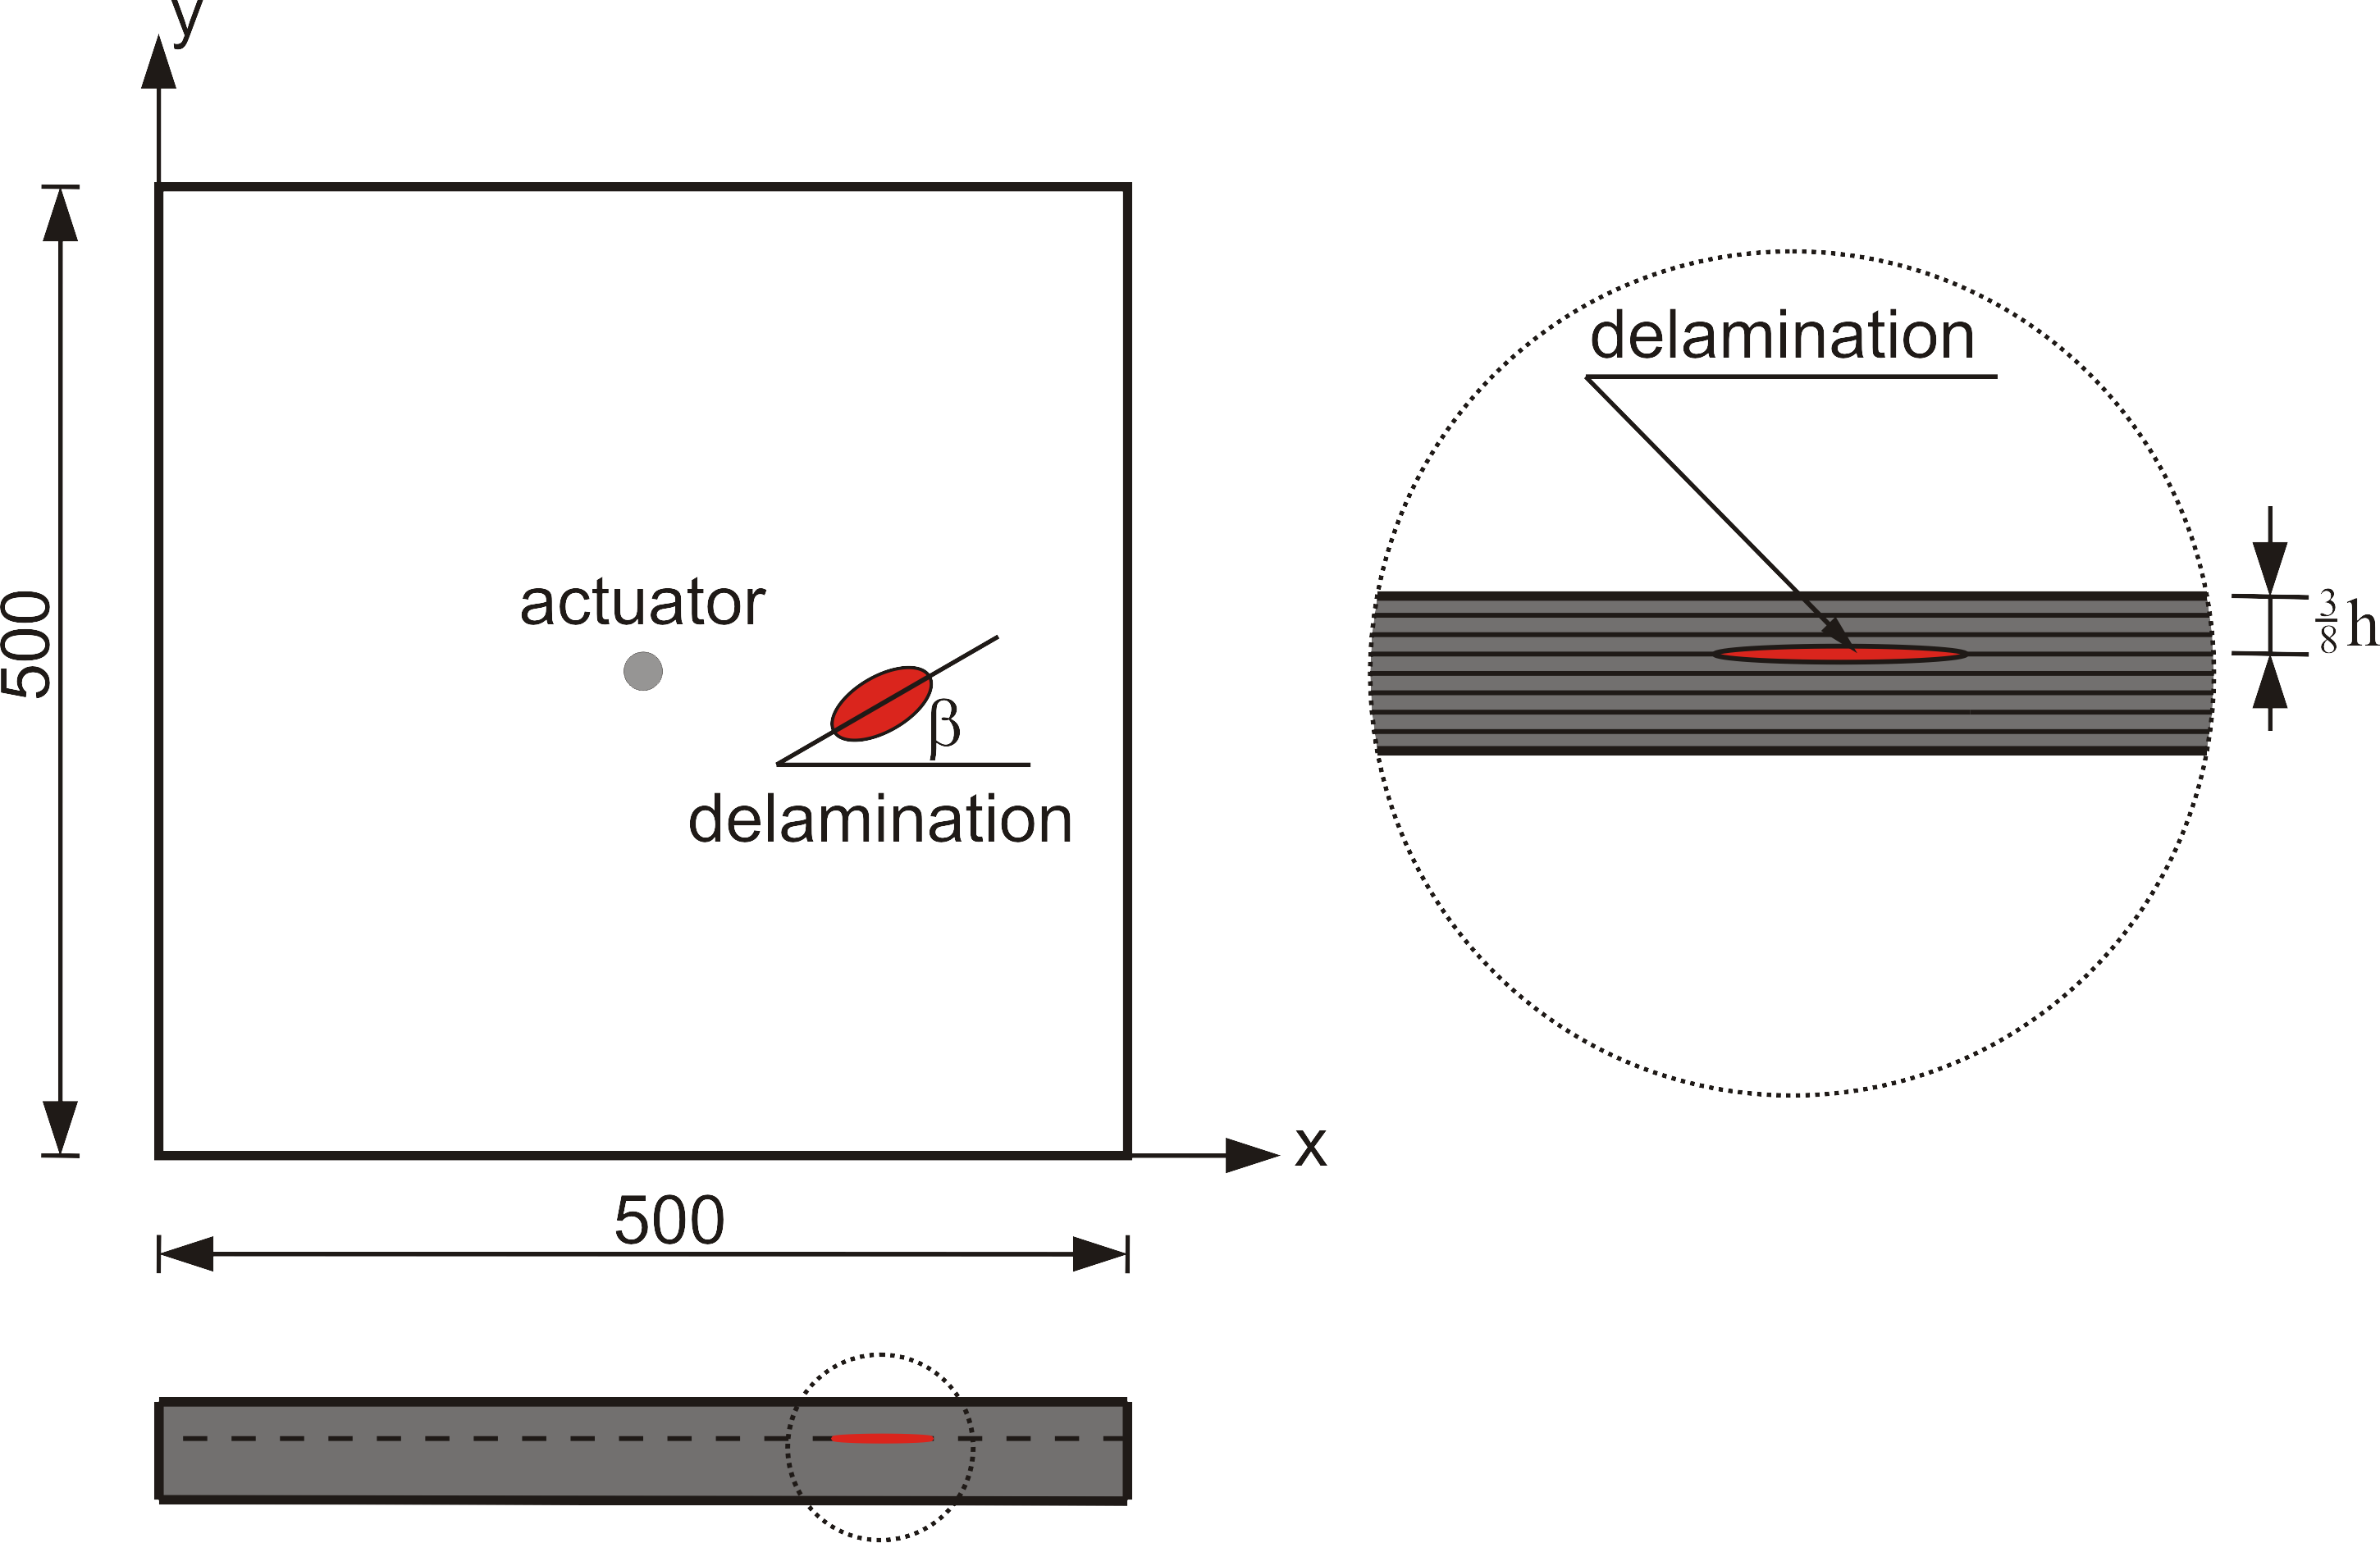
\includegraphics[scale=0.8]{Figures/Chapter_3/plate_delam_arrangement_MSSP.PNG}
	\caption{Setup for computing Lamb wave interactions with delamination.}
	\label{fig:plate_setup}
\end{figure}	
\begin{figure}
	\centering
	\includegraphics[scale=1]{Figures/Chapter_3/dataset2_labels_ellipses.png}
	\caption{The plate with 475 cases of random delaminations.}
	\label{fig:random_delam}
\end{figure}

Guided waves were excited at the plate centre by applying equivalent piezoelectric forces.
The excitation signal had a form of sinusoid modulated by Hann window. 
It was assumed that the carrier frequency is 50 kHz and the modulation frequency is 10 kHz.
A relatively low carrier frequency allowed for lower mesh density and significant computation time reduction in comparison to simulations of higher frequencies.
Additionally, the excitation signal was selected so that interaction of generated A0 Lamb wave mode with the smallest delamination can be still used as a feature for damage identification.

The output from the top and bottom surfaces of the plate in the form of particle velocities at the nodes of spectral elements were interpolated on the uniform grid of 500\(\times\)500 points by using shape functions of elements (see~\cite{Kudela2020} for more details).
It essentially resembles measurements acquired by SLDV in the transverse direction (perpendicular to the plate surface).
An example of the simulated full wavefield data on the top and bottom surfaces is presented in Fig.~\ref{fig:wavefield}.
It should be noted that stronger wave entrapment at delamination can be observed for the case of the wavefield at the top surface.
It is because the delamination within cross-section is located closer to the top surface.
It makes it easier to detect delamination by processing wavefield at the top surface.
It is better visible if the root mean square (RMS) according to Eq.~(\ref{eq:rms}) is applied to the wavefield.
The result of this operation is presented in Fig.~\ref{fig:rms}.
Based on the image analysis, the shape of the delamination can be easier to discern for the top case.
However, the methodology presented in this paper was applied to the more difficult case i.e. wavefield registered at the bottom surface of the plate.

%The dataset consisting of RMS images which were used in this research paper is available online~\cite{Kudela2020d}.

\begin{figure} [h!]
	\centering
	\begin{subfigure}[b]{0.32\textwidth}
		\centering
		\includegraphics[scale=1]{Figures/Chapter_3/96_flat_shell_Vz_1_500x500top.png}
		\caption{\(t=0.141\) ms}
		\label{fig:frame96top}
	\end{subfigure}
	\hfill
	\begin{subfigure}[b]{0.32\textwidth}
		\centering
		\includegraphics[scale=1]{Figures/Chapter_3/128_flat_shell_Vz_1_500x500top.png}
		\caption{\(t=0.188\) ms}
		\label{fig:frame128top}
	\end{subfigure}
	\hfill
	\begin{subfigure}[b]{0.32\textwidth}
		\centering
		\includegraphics[scale=1]{Figures/Chapter_3/164_flat_shell_Vz_1_500x500top.png}
		\caption{\(t=0.240\) ms}
		\label{fig:frame164top}
	\end{subfigure}	
	\hfill
	\begin{subfigure}[b]{0.32\textwidth}
		\centering
		\includegraphics[scale=1]{Figures/Chapter_3/96_flat_shell_Vz_1_500x500bottom.png}
		\caption{\(t=0.141\) ms}
		\label{fig:frame96bottom}
	\end{subfigure}
	\hfill
	\begin{subfigure}[b]{0.32\textwidth}
		\centering
		\includegraphics[scale=1]{Figures/Chapter_3/128_flat_shell_Vz_1_500x500bottom.png}
		\caption{\(t=0.188\) ms}
		\label{fig:frame128bottom}
	\end{subfigure}
	\hfill
	\begin{subfigure}[b]{0.32\textwidth}
		\centering
		\includegraphics[scale=1]{Figures/Chapter_3/164_flat_shell_Vz_1_500x500bottom.png}
		\caption{\(t=0.240\) ms}
		\label{fig:frame164bottom}
	\end{subfigure}
	
	\caption{Full wavefield at the top surface (a)--(c) and the bottom surface (d)--(f), respectively, at selected time instances showing the interaction of guided waves with delamination.}
	\label{fig:wavefield}
\end{figure} 

\begin{figure} [h!]
	\centering
	\begin{subfigure}[b]{0.47\textwidth}
		\centering
		\includegraphics[scale=1]{Figures/Chapter_3/RMS_flat_shell_Vz_1_500x500top.png}
		\caption{top}
		\label{fig:rmstop}
	\end{subfigure}
	\hfill
	\begin{subfigure}[b]{0.47\textwidth}
		\centering
		\includegraphics[scale=1]{Figures/Chapter_3/RMS_flat_shell_Vz_1_500x500bottom.png}
		\caption{bottom}
		\label{fig:rmsbottom}
	\end{subfigure}
	\caption{RMS of the full wavefield from the top surface of the plate (a) and the bottom surface of the plate (b).}
	\label{fig:rms}
\end{figure} 

%% SECTION HEADER ////////////////////////////////////////////////////////////////////////////////
\section{Delamination detection using fully connected CNN classifier}
\label{sec42}

In this section, I present my initial attempt to solve the problem of delamination detection in CFRP materials by utilising CNN models for classification purposes.

The bounding box method was used for the classification of the location of the delamination with the input as RMS (Fig.~\ref{fig:RMS_14}) and the binary representation of the delamination shape as ground truth (label shown in Fig.~\ref{fig:label_14}).
%%%%%%%%%%%%%%%%%%%%%%%%%%%%%%%%%%%%%%%%%%%%%%%%%%%%%%%%%%%%%%%%%%%%%%%%%%%%%%%%
\begin{figure} [!ht]
	\centering
	\begin{subfigure}[b]{0.47\textwidth}
		\centering
		\includegraphics[width=5cm]{Figures/Chapter_4/RMS_flat_shell_Vz_389_500x500top.png}
		\caption{}
		\label{fig:RMS_14}
	\end{subfigure}
	\hfill
	\begin{subfigure}[b]{0.47\textwidth}
		\centering
		\includegraphics[width=5cm]{Figures/Chapter_4/m1_rand_single_delam_389.png}
		\caption{}
		\label{fig:label_14}
	\end{subfigure}
	\caption{(a) RMS image: from the top of the plate, (b) Label.}
	\label{fig:RMS_GT}
\end{figure} 
%%%%%%%%%%%%%%%%%%%%%%%%%%%%%%%%%%%%%%%%%%%%%%%%%%%%%%%%%%%%%%%%%%%%%%%%%%%%%%%%

Accordingly, CNN models with fully connected dense layers were developed for delamination detection in CFRP.
Moreover, the developed models are based on supervised learning to perform a classification task, therefore for each generated case of delamination a ground truth (label) is given.
 
\subsection{Data preprocessing}
\label{sec421}
In order to reduce the computation complexity for the model, the dataset for training the model was prepared by resizing the RMS input image to \((448\times 448)\) pixels.  
Then, it was split into \((14\times 14)\) patches, and each patch has a size of \((32\times 32)\) pixels as shown in Fig.~\ref{fig:RMS_49patches}.
Consequently, the preprocessed dataset has a size of \((93100\times 32\times 32 \times 1)\), where (\(93100\)) is the total number of patches for all \(475\) cases.

To investigate the effect of increasing the resolution of RMS images over delamination identification, I made another preparation by upsampling the RMS input image to \((512\times 512)\) pixels with cubic interpolation. Then the upsampled RMS image was split into \(16\times 16\) patches, and each patch has a size of \((32\times 32)\) pixels as shown in Fig.~\ref{fig:RMS_64patches}.
The second preprocess dataset has a size of \((121600 \times 32 \times 32 \times 1)\), where (\(121600\)) is the total number of patches for all \(475\) cases.
For each patch in the RMS input image, there is a corresponding patch in the ground truth image of size \((32\times 32)\) as presented in Figs.~\ref{fig:GT_49patches} and~\ref{fig:GT_64patches}, respectively.

For training purposes, the dataset was divided into two portions: \(80\%\)	training set and \(20\%\) testing set. 
Additionally, the validation set was created as a \(20\%\) of the training set.
%%%%%%%%%%%%%%%%%%%%%%%%%%%%%%%%%%%%%%%%%%%%%%%%%%%%%%%%%%%%%%%%%%%%%%%%%%%%%%%%
\begin{figure} [h!]
	\centering
	\begin{subfigure}[b]{0.47\textwidth}
		\centering
		\includegraphics[width=5cm]{Figures/Chapter_4/7_7_patches_389.png}
		\caption{RMS image splitted into (\(14\times 14\)) patches.}
		\label{fig:RMS_49patches}
	\end{subfigure}
	\hfill
	\begin{subfigure}[b]{0.47\textwidth}
		\centering
		\includegraphics[width=5cm]{Figures/Chapter_4/8_8_patches_389.png}
		\caption{RMS image splitted into (\(16\times 16\)) patches.}
		\label{fig:RMS_64patches}
	\end{subfigure}
	\hfill
	\begin{subfigure}[b]{0.47\textwidth}
		\centering
		\includegraphics[width=5cm]{Figures/Chapter_4/GT_7_7_389.png}
		\caption{Label image splitted into (\(14\times 14\)) patches.}
		\label{fig:GT_49patches}
	\end{subfigure}
	\hfill
	\begin{subfigure}[b]{0.47\textwidth}
		\centering
		\includegraphics[width=5cm]{Figures/Chapter_4/GT_8_8_389.png}
		\caption{Label image splitted into (\(16\times 16\)) patches.}
		\label{fig:GT_64patches}
	\end{subfigure}
	\caption{Data preparation for bounding box method.}
	\label{fig:grid_mesh}
\end{figure}
%%%%%%%%%%%%%%%%%%%%%%%%%%%%%%%%%%%%%%%%%%%%%%%%%%%%%%%%%%%%%%%%%%%%%%%%%%%%%%%%

\subsection{CNN classification models}
\label{sec422}
The architecture of the implemented CNN model for classification purposes is presented in Fig.~\ref{CNN_model}.
The model takes an input patch of size \((32\times 32)\) pixels, followed by a convolutional layer that has (\(64\)) filters of size (\(3\times 3\)).
Moreover, in the convolution operation, the padding was set to be the same,  and the activation function was Relu.
Then, a pooling layer is applied, which has a pool filter of size (\(2\times 2\)) with a stride of (\(2\)).
This operation of convolution and pooling is repeated two times.
The output of the second pooling layer is flattened and fed into the dense layers in which the model has two fully connected layers.
The first dense layer has (\(4096\)) neurons, and the second dense layer has (\(1024\)) neurons.
A dropout of probability (\(p = 0.5\)) was added to the model to reduce the overfitting issue.

Moreover, selecting a proper objective function (loss) during training is important as the loss function reflects how well the model learns to predict.
Hence, I have applied the mean square error \((MSE)\) loss function depicted in Eqn.~\ref{mse}, which calculates the sum of the squared distances between the predicted output values and the ground truth values:
\begin{equation}
	MSE=\frac{1}{M*N}\sum_{M,N}^{}(Y_{(m,n)}-\hat{Y}_{(m,n)})^2,
	\label{mse}
\end{equation}
where \(M\) and \(N\) are the number of rows and columns in the input images, \(Y_{(m,n)}\) is the ground truth value, and \(\hat{Y}_{(m,n)}\) is the predicted value.

The final layer in the model is the output layer, in which the model outputs two predictions (damaged and undamaged).
Hence, the softmax activation function was used, which estimates the probability of each predicted output as being damaged or undamaged, implying that the sum of the two probabilities must be one.
The reason behind choosing the softmax at the output layer is to avoid thresholding of the predicted output (e.g. a sigmoid produces values in a range between (\(0\) and \(1\))).
The softmax activation function is depicted by Eq.~(\ref{softmax}): 
\begin{equation}
	P(x)_{i} = \frac{e^{x_{i}}}{\sum_{j}^{C} e^{x_{j}}}.
	\label{softmax}
\end{equation} 
where \(P(x)_{i}\) is the probability of each target class \(x_{j}\) across all potential target classes \(x_{j}\), C in our instance being two classes (damaged and undamaged).

Additionally, an argmax function is used to find the maximum probability between each of them in order to predict the label of the output (\(y_{pred}\)).
Equation~\ref{argmax} depicts the argmax function.
\begin{equation}
	y_{pred} = \mathrm{argmax}_{i}\left( P(x)_{i} \right)
	\label{argmax}
\end{equation}

Accordingly, the whole patch of size \((32\times 32)\) is classified as damaged if there is at least one pixel of delamination, otherwise, it is considered undamaged.
Finally, the predicted output (delamination) is surrounded by a bounding box as the final output.
%%%%%%%%%%%%%%%%%%%%%%%%%%%%%%%%%%%%%%%%%%%%%%%%%%%%%%%%%%%%%%%%%%%%%%%%%%%%%%%%
\begin{figure}[h!]
	\centering
	\includegraphics[scale=1]{Figures/Chapter_4/CNN_model.png}
	\caption{CNN classifier architecture.}
	\label{CNN_model}
\end{figure}
%%%%%%%%%%%%%%%%%%%%%%%%%%%%%%%%%%%%%%%%%%%%%%%%%%%%%%%%%%%%%%%%%%%%%%%%%%%%%%%%

%% SECTION HEADER ////////////////////////////////////////////////////////////////////////////////
\section{FCN models for delamination identification}
\label{sec43}
DL approaches have advanced quickly in recent years in many different real-world applications.
An important and challenging application among others in DL is computer vision, in which we train a machine to automatically extract useful information from digital images, videos, and other visual inputs.
Hence, an image segmentation technique that is well-known in computer vision applications is broadly utilised for such a purpose.
Consequently, this technique aims to assign a class to each pixel in the input image.
Thus, it can be utilised in several real-world applications like self-driving automobiles, medical imaging, traffic management systems, video surveillance, and more.
%%%%%%%%%%%%%%%%%%%%%%%%%%%%%%%%%%%%%%%%%%%%%%%%%%%%%%%%%%%%%%%%%%%%%%%%%%%%%%%%

In this section, I present five DL models based on Fully Convolutional Networks (FCN)~\cite{Shelhamer2017} that aim to automatically perform feature extraction by training the models using full wavefield images. 
Therefore, the models will learn by themselves to recognise the different patterns further, detect the delamination and localise it.
Consequently, the implemented models will perform a pixel-wise segmentation by classifying every pixel of the input image as damaged or not.

The key idea of FCN is to replace the dense layers of neurons with convolutional layers, hence, reducing the computation complexity.
Hence, FCN can be implemented by stacking convolutional layers and skipping dense layers in an encoder-decoder scheme.
The encoder aims to produce compressed feature maps from the input image at various scale levels using cascaded convolutions and downsampling operations.
While the decoder is responsible for upsampling the condensed feature maps to the original input shape.

The softmax function (see Eqn.~\ref{softmax}) was used at the output layer for all developed FCN models.
Additionally, the categorical cross-entropy (CCE) loss function~\cite{Bonaccorso2020}, commonly known as the \enquote{softmax loss function}, was utilised in all FCN models.
The difference between the actual damage (ground truth) and the expected damage is estimated using CCE as the objective function.
The CCE is illustrated by Eq.~(\ref{CCE}), where \( P(x)_{i}\) refers to the softmax value of the target class:
\begin{equation}	
	CCE = -\log\left( P(x)_{i} \right).
	\label{CCE}
\end{equation}

It should be noted, as there are only two classes to predict, a Sigmoid activation function at the output layer can be combined with a binary cross-entropy (BCE) without affecting the predicted outputs.

The implemented DL models for pixel-wise semantic segmentation for delaminations identification are depicted in Figure~\ref{fig:flowchart}.
In the following subsections~(\ref{sec431}~-~\ref{sec436}), the data preprocessing and the five DL models will be illustrated.
%%%%%%%%%%%%%%%%%%%%%%%%%%%%%%%%%%%%%%%%%%%%%%%%%%%%%%%%%%%%%%%%%%%%%%%%%%%%%%%%
\begin{figure} [h!]
	\begin{center}
		\includegraphics[scale=1.0]{Figures/Chapter_4/figure3.png}
	\end{center}
	\caption{Schematic diagram of the approach used for comparison of semantic segmentation methods accuracy.} 
	\label{fig:flowchart}
\end{figure}
%%%%%%%%%%%%%%%%%%%%%%%%%%%%%%%%%%%%%%%%%%%%%%%%%%%%%%%%%%%%%%%%%%%%%%%%%%%%%%%%
\subsection{Data preprocessing}
\label{sec431}
%%%%%%%%%%%%%%%%%%%%%%%%%%%%%%%%%%%%%%%%%%%%%%%%%%%%%%%%%%%%%%%%%%%%%%%%%%%%%%%%
The implemented FCN models for pixel-wise image segmentation have a one-to-one prediction scheme.
In other words, the models take one image input and predict one output image.
Accordingly, to train the FCN models, the calculated RMS images of the full wavefield at the bottom surface of the plate (see Fig.~\ref{fig:rmsbottom}) were utilised.
The dataset consisting of RMS images which were used in this research paper is available online~\cite{Kudela2020d}.

To enhance the performance of the optimizer during the training process, the colour scale values were normalised to a range of \((0-1)\) instead of the initial scale which was in a range of \((0-255)\). 
Furthermore, I have applied data augmentation to the dataset (\(475\) RMS images) by flipping the images horizontally, vertically, and diagonally. 
As a result, the dataset size increased four times -\(1900\) images were produced. 
I have split the dataset into two portions: \(80\%\) for the training set and \(20\%\) for the testing set. 
Moreover, a K-folds cross-validation technique~\cite{Srinivasan2019} was applied to the training set to reduce the overfitting which happens when the model is able to fit on the training data, while it poorly fit on the new unseen data.
In other words, the model only learns the patterns of the training data therefore the model will not generalise well. 
The main advantage of the K-folds method versus a regular train/test split is to reduce the overfitting by utilising data more efficiently as every data sample is used in both training and validation. 
Therefore, by using this technique, I aim to improve the ability of the model to generalise and reduce overfitting.
Figure~\ref{fig:cross_validation} illustrates the K-folds cross validation technique.
%%%%%%%%%%%%%%%%%%%%%%%%%%%%%%%%%%%%%%%%%%%%%%%%%%%%%%%%%%%%%%%%%%%%%%%%%%%%%%%%
\begin{figure} [h!]
	\begin{center}
		\includegraphics[scale=1.0]{Figures/Chapter_4/cross_validation.png}
	\end{center}
	\caption{K-folds cross validation.} 
	\label{fig:cross_validation}
\end{figure}
%%%%%%%%%%%%%%%%%%%%%%%%%%%%%%%%%%%%%%%%%%%%%%%%%%%%%%%%%%%%%%%%%%%%%%%%%%%%%%%%
%%%%%%%%%%%%%%%%%%%%%%%%%%%%%%%%%%%%%%%%%%%%%%%%%%%%%%%%%%%%%%%%%%%%%%%%%%%%%%%%
\subsection{Residual UNet model}
\label{sec432}
%%%%%%%%%%%%%%%%%%%%%%%%%%%%%%%%%%%%%%%%%%%%%%%%%%%%%%%%%%%%%%%%%%%%%%%%%%%%%%%%
The Residual UNet (Res-UNet) model was inspired based on residual learning~\cite{He2016} and UNet approaches~\cite{Ronneberger2015}.
The Res-UNet architecture is depicted in Fig.~\ref{fig:Unet}.
The encoder (compressive) path aims to capture the detailed features of an input image, whereas the decoder (decompressive) path aims to perform exact localization.
As a result, residual connections were established at two levels in order to prevent the spatial and contextual information from the preceding layers from being lost:

\begin{itemize}
	\item at each step of the encoder and decoder paths,
	\item between the encoder parts and their corresponding decoder parts (skip connections) which ensures that the feature maps which were learned during the downsampling will be utilized in the reconstruction. 
\end{itemize}

%%%%%%%%%%%%%%%%%%%%%%%%%%%%%%%%%%%%%%%%%%%%%%%%%%%%%%%%%%%%%%%%%%%%%%%%%%%%%%%%
Several downsampling (Max-pool) blocks are used in the encoder section.
Each block applies two convolutional layers followed by a (\(2\times2\)) max pooling with a (\(2\times2\)) strides that selects the maximum value in a local pool filter in one feature map (or \(n\)-feature maps), resulting in a reduction in the dimension of feature maps~\cite{Lecun2015}, and in turn, a reduction in computation complexity.
Each convolutional layer does \((3\times3)\) convolution operations, then batch normalization (BN), and finally a Relu.
Furthermore, after each downsampling block, the number of convolutional filters is increased, allowing the model to learn complex patterns successfully.
%%%%%%%%%%%%%%%%%%%%%%%%%%%%%%%%%%%%%%%%%%%%%%%%%%%%%%%%%%%%%%%%%%%%%%%%%%%%%%%%

The bottleneck layer is a joining point in the model's deepest layer, located between the encoder and the decoder.
Two convolutional layers with \((1024)\) filters make up the bottleneck, which aids the model in learning and recognizing complex features.
%%%%%%%%%%%%%%%%%%%%%%%%%%%%%%%%%%%%%%%%%%%%%%%%%%%%%%%%%%%%%%%%%%%%%%%%%%%%%%%%

The decoder is composed of a number of upsampling blocks that function together to recover original input dimensions and improve resolution.
As in the downsampling block, each upsampling block transmits the input through two convolution layers, followed by a transmission up layer consisting of a transposed convolutional layer (upsampling).
The transposed convolutional layer varies from the standard upsampling function in that it introduces learnable parameters for the transposed convolution filters, which improve the model's learning process.
Furthermore, the number of filters used by the convolutional layer is reduced by half after each upsampling operation to keep the model symmetrical.
%%%%%%%%%%%%%%%%%%%%%%%%%%%%%%%%%%%%%%%%%%%%%%%%%%%%%%%%%%%%%%%%%%%%%%%%%%%%%%%%
\begin{figure} [h!]
	\begin{center}
		\includegraphics[width=\textwidth]{Figures/Chapter_4/figure4.png}
	\end{center}
	\caption{Res-UNet architecture.} 
	\label{fig:Unet}
\end{figure}
%%%%%%%%%%%%%%%%%%%%%%%%%%%%%%%%%%%%%%%%%%%%%%%%%%%%%%%%%%%%%%%%%%%%%%%%%%%%%%%%
\subsection{VGG16 encoder-decoder}
\label{sec433}
%%%%%%%%%%%%%%%%%%%%%%%%%%%%%%%%%%%%%%%%%%%%%%%%%%%%%%%%%%%%%%%%%%%%%%%%%%%%%%%%
The application of the VGG16~\cite{Simonyan2015} architecture as a backbone encoder to the UNet~\cite{Ronneberger2015} approach is addressed in this model.
VGG16 is a classification algorithm that consists of 13 convolutional layers, pooling layers, and (3) dense layers.
The dense layers were removed form the original VGG16 model, and a 13 convolutional layers were applied resulting in an encoder-decoder scheme for pixel-wise image segmentation.
The architecture of the VGG16 encoder-decoder model is shown in Fig.~\ref{vgg16}.
The model is U-shaped like, and consists of two parts: encoder and decoder.
The encoder is made up of (five) convolutional blocks with a total of (13) \((3\times3)\) convolutional layers, followed by BN and Relu as the activation function.
After each convolutional block, a Max pool operation with a pool size of \((2\times2)\) is conducted, followed by dropout. 
The upsampling process is used to retrieve spatial resolution, and it contains \(5\) convolutional blocks of total \(13\) convolutional layers.
Bilinear interpolation with \((2\times2)\) kernel size is used for upsampling.
In order to improve recovering fine-grained information, skip connections were added between downsampling blocks and the matching upsampling blocks, allowing feature re-usability from earlier layers.
\begin{figure} [h!]
	\begin{center}
		\includegraphics[width=\textwidth]{Figures/Chapter_4/figure5.png}
	\end{center}
	\caption{VGG16 encoder decoder architecture.} 
	\label{vgg16}
\end{figure}

%%%%%%%%%%%%%%%%%%%%%%%%%%%%%%%%%%%%%%%%%%%%%%%%%%%%%%%%%%%%%%%%%%%%%%%%%%%%%%%%
\subsection{FCN-DenseNet model}
\label{sec434}
%%%%%%%%%%%%%%%%%%%%%%%%%%%%%%%%%%%%%%%%%%%%%%%%%%%%%%%%%%%%%%%%%%%%%%%%%%%%%%%%
FCN-DenseNet is a pixel-wise image segmentation algorithm that was first introduced in~\cite{Jegou}.
To boost the resolution of the final feature map, FCN-DenseNet uses a U-shaped encoder-decoder architecture with skip connections between downsampling and upsampling channels.
Hence, FCN-DenseNet introduced a dense block representing its main component.
The dense block is made up of \(n\) layers, each of which is made up of a set of operations, as given in Table~\ref{layers}.
The purpose of the dense block is to concatenate the input (feature maps) of a layer with its output (feature maps) to emphasize spatial details information.
The architecture of the dense block is presented in Fig.~\ref{dense_block}. 
\begin{figure} [h!]
	\begin{center}
		\includegraphics[width=0.5\textwidth,angle=-90]{Figures/Chapter_4/figure6.png}
	\end{center}
	\caption{Dense block architecture.} 
	\label{dense_block}
\end{figure}
%%%%%%%%%%%%%%%%%%%%%%%%%%%%%%%%%%%%%%%%%%%%%%%%%%%%%%%%%%%%%%%%%%%%

A transition down layer was added to execute a \((1\times 1)\) convolution followed by a \((2\times 2)\) Maxpooling operation to minimize the spatial dimensionality of the resulting feature maps.
As a result, a transition-up layer was added to recover the spatial resolution.
FCN-DenseNet essentially upsamples feature maps from the previous layer using a transpose convolution technique.
Upsampled feature maps are concatenated with those produced by the skip connection to provide the input to a new dense block.

As the upsampling approach expands the spatial resolution of the feature maps, the input to the dense block is not concatenated with its output during upsampling to avoid the overhead of memory shortage.
The FCN-DenseNet architecture for image segmentation utilized for delamination detection is shown in Fig.~\ref{fcn}.
%%%%%%%%%%%%%%%%%%%%%%%%%%%%%%%%%%%%%%%%%%%%%%%%%%%%%%%%%%%%%%%%%%%%%%%%%%%%%%%%
\begin{figure} [h!]
	\begin{center}
		\includegraphics[width=.7\textwidth]{Figures/Chapter_4/FCN_dense_net.png}
	\end{center}
	\caption{FCN-DenseNet architecture.} 
	\label{fcn}
\end{figure}
%%%%%%%%%%%%%%%%%%%%%%%%%%%%%%%%%%%%%%%%%%%%%%%%%%%%%%%%%%%%%%%%%%%%%%%%%%%%%%%%
Table~\ref{layers} presents the architecture of a single layer, the transition down and transition up layers in details.
%%%%%%%%%%%%%%%%%%%%%%%%%%%%%%%%%%%%%%%%%%%%%%%%%%%%%%%%%%%%%%%%%%%%
\begin{table}[h!]
	\renewcommand{\arraystretch}{1.3}
	\centering
	\scriptsize
	\resizebox{\textwidth}{!}
	{
		\begin{tabular}{ccccc}
			\hline
			Layer & & Transition Down & & Transition Up \\ 
			\hline
			Batch Normalization & & Batch Normalization & & \(3\times 3\) Transposed Convolution \\ 
			Relu & & Relu & & strides = (\(2\times2\)) \\ 
			(\(3\times3\)) Convolution & & (\(1\times1\)) Convolution & & \\ 
			%		& &  \\ 
			Dropout \(p=0.2\) & &Dropout \(p=0.2\) & & \\ 
			& & (\(2\times2\)) Maxpooling & & \\ 
			\hline
		\end{tabular}
	}
	\caption{Layer, Transition Down and Transition Up layers.} 
	\label{layers}	
\end{table}\\
%%%%%%%%%%%%%%%%%%%%%%%%%%%%%%%%%%%%%%%%%%%%%%%%%%%%%%%%%%%%%%%%%%%%%%%%%%%%%%%%
\subsection{Pyramid Scene Parsing Network}
\label{sec435}
%%%%%%%%%%%%%%%%%%%%%%%%%%%%%%%%%%%%%%%%%%%%%%%%%%%%%%%%%%%%%%%%%%%%%%%%%%%%%%%%
The main idea of PSPNet~\cite{zhao2017pyramid} is to combine local and global features to give appropriate global contextual information for pixel-level scene parsing.
As a result, a spatial pyramid pooling module was developed to execute four different layers of pooling with four different pooling sizes and strides.
The pyramid pooling module is able to capture contextual features from many scales in this way.

To enhance the PSPNet model a ResNet-50 model~\cite{He2016} was added. 
It works as a backbone for feature map extraction with dilation at the last two layers of ResNet. 
The implemented PSPNet architecture is shown in Fig.~\ref{fig:PSPNet}.
Hence, a pyramid pooling module was utilised at \(4\) pooling levels.
The coarsest level of a single bin output depicted in the red box was generated using global average pooling.
(\(2\times2\)), (\(4\times 4\)), and (\(8\times8\)) are the pooling sizes for the other three sub-region levels, respectively.
To minimize the dimensionality of the generated feature maps, a \((1\times 1)\) convolutional layer was applied, followed by a BN and Relu.
Subsequently, bilinear interpolation was used to upsample the feature maps created at each level.
Furthermore, the upsampled features are combined with the output of ResNet-50 to produce both local and global context information.
The pixel-wise segmentation predictions were then generated using two cascaded convolutional layers. 
\begin{figure} [h!]
	\centering
	\includegraphics[width=.8\textwidth]{Figures/Chapter_4/figure7.png}
	\caption{PSPNet architecture.} 
	\label{fig:PSPNet}
\end{figure} 
%%%%%%%%%%%%%%%%%%%%%%%%%%%%%%%%%%%%%%%%%%%%%%%%%%%%%%%%%%%%%%%%%%%%%%%%%%%%%%%%
\subsection{Global Convolutional Network}
\label{sec436}
%%%%%%%%%%%%%%%%%%%%%%%%%%%%%%%%%%%%%%%%%%%%%%%%%%%%%%%%%%%%%%%%%%%%%%%%%%%%%%%%
Peng et al.~\cite{Peng2017} introduced the Global Convolutional Network (GCN) to address the importance of having large kernels for both localization and classification operations for semantic segmentation in order to increase the size of respective fields.
However, when performing classification and localization tasks, a contradiction emerges due to the fact that classification tasks necessitate invariant models for various transformations such as rotation and translation while localisation tasks necessitate models that are sensitive to any modification and appropriately assign each pixel to its semantic category.
To alleviate such contradiction, two design principles were proposed:
\((1)\) For the classification task, in order to improve the capability of 
the model to handle different transformations, a large kernel size must be 
used to enable dense connections between feature maps and per-pixel 
classifiers; \((2)\) for localisation task, the model must be fully convolutional. 
Additionally, fully connected or global pooling layers are not applied as 
these layers will discard the localisation information. 

The implemented GCN technique for semantic segmentation is shown in Fig.~\ref{fig:gcn}.
%%%%%%%%%%%%%%%%%%%%%%%%%%%%%%%%%%%%%%%%%%%%%%%%%%%%%%%%%%%%%%%%%%%%%%%%%%%%%%%%
\begin{figure} [h!]
	\begin{center}
		\includegraphics[width=.8\textwidth]{Figures/Chapter_4/figure8.png}
	\end{center}
	\caption{Global Convolution Network whole architecture.} 
	\label{fig:gcn}
\end{figure}
%%%%%%%%%%%%%%%%%%%%%%%%%%%%%%%%%%%%%%%%%%%%%%%%%%%%%%%%%%%%%%%%%%%%%%%%%%%%%%%%

A residual network was used as a backbone for improving the feature extraction process, as demonstrated in Fig.~\ref{fig:gcn}, further, the residual block is presented in Fig.~\ref{fig:res_gcn_br}a.
A GCN block presented in Fig.~\ref{fig:res_gcn_br}b is placed after each residual block, which employs a mix of \((1\times k)\)+\((k\times 1)\) and \((k\times 1)\)+\((1\times k)\) convolutions to establish dense connections within \((k\times k)\) region in the feature map.
The boundary refinement (BR) block, depicted in Fig.~\ref{fig:res_gcn_br}c, is then used to improve the predictions along the object borders, resulting in a lower resolution score map.
Furthermore, the upsampling operation is done recursively. 
It upsamples the low resolution score maps then concatenate it with a higher one to produce a new 
score maps.
The deconvolution operation is repeated until the original image size is 
obtained.
\begin{figure} [h!]
	\begin{center}
		\includegraphics[width=.8\textwidth]{Figures/Chapter_4/figure9.png}
	\end{center}
	\caption{(a) Residual block, (b) Global Convolution Network block, (c) 
		Boundary Refinement} 
	\label{fig:res_gcn_br}
\end{figure}

\section{Convergence of FCN models}


\begin{figure} [h!]
	\centering
	\begin{subfigure}[b]{0.49\textwidth}
		\centering
		\includegraphics[width=1\textwidth]{Figures/Chapter_4/UNet_loss.png}
		\caption{}
		\label{fig:UNet_loss}
	\end{subfigure}
	\hfill
	\begin{subfigure}[b]{0.49\textwidth}
		\centering
		\includegraphics[width=1\textwidth]{Figures/Chapter_4/VGG16_loss.png}
		\caption{}
		\label{fig:VGG16_loss}
	\end{subfigure}
	\hfill
	\begin{subfigure}[b]{0.49\textwidth}
		\centering
		\includegraphics[width=1\textwidth]{Figures/Chapter_4/FCN_densenet_loss.png}
		\caption{}
		\label{fig:FCN_densenet_loss}
	\end{subfigure}	
	\hfill
	\begin{subfigure}[b]{0.49\textwidth}
		\centering
		\includegraphics[width=1\textwidth]{Figures/Chapter_4/PSPNET_loss.png}
		\caption{}
		\label{fig:PSPNet_loss}
	\end{subfigure}
	\begin{subfigure}[b]{0.49\textwidth}
		\centering
		\includegraphics[width=1\textwidth]{Figures/Chapter_4/GCN_loss.png}
		\caption{}
		\label{fig:GCN_loss}
	\end{subfigure}
	\caption{}
	\label{fig:FCN_model_convergence}
\end{figure} 
\clearpage

%% SECTION HEADER /////////////////////////////////////////////////////////////////////////////////////
\section{Delamination identification using FCN}
\label{sec44}

%% SECTION HEADER ////////////////////////////////////////////////////////////////////////////////
\section{Super-Resolution image reconstruction for delamination identification}
\label{sec45}
Guided waves, in particular Lamb waves, are often utilised for structural health monitoring (SHM) as well as non-destructive testing (NDT).
In the former case, usually an array of transducers is used for point-wise measurements.
These are usually piezoelectric transducers that can work as actuators and sensors, i.e. in active guided wave-based SHM.
It should be noted that round-robin actuator-sensor measurements can be conducted very fast, therefore nearly online monitoring of a structure is possible.

Recently, a lot of research on the application of scanning laser Doppler vibrometer (SLDV) for NDT is reported~\cite{Flynn2013,Kudela2015,Kudela2018d,Segers2021,Segers2022}. 
In this method, either piezoelectric transducer or pulse laser is used for guided wave excitation while the measurements are taken by SLDV at one point on the surface of an inspected structure.
The process is repeated for other points automatically in a scanning fashion until full wavefield of Lamb waves is acquired.

Full wavefield measurements are taken on a very dense grid of points opposite to sparsely measured signals by sensors.
Hence, deliver much more useful data from which information about damage can be extracted in comparison to signals measured by an array of transducers.
On the other hand, SLDV measurements take much more time than measurements conducted by an array of transducers.
It makes the SLDV approach unsuitable for SHM in which continuous monitoring is required.
But it is very capable for offline NDT applications.

One can imagine that in a future matrix of laser heads instead of a single laser head used nowadays will be developed to reduce SLDV measurement time.
Alternatively, compressive sensing (CS) and/or deep learning super-resolution (DLSR) can be applied.
It means that SLDV measurements can be taken on a low-resolution grid of points and then full wavefield can be reconstructed at high-resolution.

CS was originally proposed in the field of statistics~\cite{Candes2006,Donoho2006} and used for efficient acquisition and reconstruction of signals and images.
It assumes that a signal or an image can be represented in a sparse form in another domain with appropriate bases (Fourier, cosine, wavelet).
On such bases, many coefficients are close or equal to zero.
The sparsity can be exploited to recover a signal or image from fewer samples than required by the Nyquist–Shannon sampling theorem.
However, there is no unique solution for the estimation of unmeasured data.
Therefore, optimisation methods for solving under-determined systems of linear equations that promote sparsity are applied~\cite{Chen1998,VanEwoutBerg2008,VandenBerg2019}.
Moreover, a suitable sampling strategy is required.

Since then, CS has found applications in medical imaging~\cite{Lustig2007}, communication systems~\cite{Gao2018}, and seismology~\cite{Herrmann2012}.
It is also considered in the field of guided waves and ultrasonic signal processing~\cite{Harley2013,Mesnil2016,Perelli2012,Perelli2015,DiIanni2015,KeshmiriEsfandabadi2018,Chang2020}

Harley and Mura~\cite{Harley2013} utilised a general model for Lamb waves propagating in a plate structure (without defects) and $L_1$ optimisation strategies to recover their frequency-wavenumber representation. 
They applied sparse recovery by basis pursuit and sparse wavenumber synthesis.
They used a limited number of transducers and achieved a good correlation between the true and estimated responses across a wide range of frequencies.
Mensil and Ruzzene~\cite{Mesnil2016} were focused on the reconstruction of wavefield that includes the interaction of Lamb waves with delamination.
Similar to previous studies, analytic solutions were utilised to create a compressive sensing matrix.
However, the limitation of these methods is that dispersion curves of Lamb waves propagating in the analysed plate have to be known a priori.

Perelli et al.~\cite{Perelli2012} incorporated the warped frequency transform into a compressive sensing framework for improved damage localisation.
The wavelet packet transform and frequency warping was used in~\cite{Perelli2015} to generate a sparse decomposition of the acquired dispersive signal.

Di Ianni et al.~\cite{DiIanni2015} investigated various bases in compressive sensing to reduce the acquisition time of SLDV measurements.
Similarly, a damage detection and localisation technique based on a compressive sensing algorithm was presented in~\cite{KeshmiriEsfandabadi2018}.
The authors have shown that the acquisition time can be reduced significantly without losing detection accuracy.

Another application of compressive sensing was reported in~\cite{Chang2020}. 
The authors used signals registered by an array of sensors for tomography of corrosion.
They investigated the reconstruction success rate depending on the number of actuator-sensor paths.

The group of DLSR methods is applied mostly to images~\cite{Dahl2017,Zhang2018,Wang2019} and videos~\cite{Zhang2017,Yan2019}.
Image super-resolution (SR) is the process of recovering high-resolution images from low-resolution images.
A similar approach can be used in videos where data is treated as a sequence of images.
Notable applications are medical imaging, satellite imaging, surveillance and security, astronomical imaging, amongst others.
Also deep learning super sampling developed by Nvidia and FidelityFX super-resolution developed by AMD was adopted for video games~\cite{Claypool2006}.
Mostly supervised techniques are employed
which benefit from recent advancements in deep learning methods ranging from enhanced convolutional neural networks (CNN)~\cite{Zhang2017}, through an extension of PixelCNN~\cite{Dahl2017} to generative adversarial networks (GANs)~\cite{Wang2019}, to name a few.
Nevertheless, so far neither of these methods have been applied to wavefields of propagating Lamb waves.
The exception is an enhancement of wavefields as the second step of SR followed by classic CS~\cite{Park2017a,KeshmiriEsfandabadi2020}.

We propose a framework for full wavefield reconstruction of propagating Lamb waves from spatially sparse SLDV measurements of resolution below the Nyquist wavelength $\lambda_N$. 
The Nyquist wavelength is the shortest spatial wavelength that can be accurately recovered from wavefield by sequential observations with spacing $\Delta x$ which is defined as $\lambda_N = 2 \Delta x$. 

For the first time, an end-to-end approach for SR problem is used in which deep learning neural network is trained on a synthetic dataset and tested on experimental data acquired by SLDV.
It means that the approach is solely based on DLSR.
It is different from methods presented in the literature which utilize CS theory~\cite{Harley2013,KeshmiriEsfandabadi2018} or CS theory in conjunction with super-resolution convolutional neural networks for wavefield image enhancement~\cite{Park2017a,KeshmiriEsfandabadi2020}.
The efficacy of the developed framework is presented and compared with conventional CS approach.  
The performance of the proposed technique is validated by an experiment performed on a plate made of carbon fibre reinforced polymer (CFRP) with embedded Teflon inserts simulating delaminations.

\subsection{Dataset preparation}
\label{sec62}
In order to train deep learning models to perform super-resolution image reconstruction, I have to reproduce a low-resolution training set from the original high-resolution dataset. 
Initially, I have resized the frames in the original high-resolution dataset to \((512\times512)\) pixels to obtain the desired output frame shape while preforming image reconstruction from the low- to high-resolutions.

In this work, I have generated a low-resolution training set with a frame size \((32\times32)\) pixels, which is below the Nyquist sampling rate of a 2D frame.
Hence, I have performed image subsampling with bi-cubic interpolation and a uniform mesh of size \((32\times32)\) pixels with a compression rate (CR) of \(21.5\%\) from the Nyquist sampling rate as depicted in Eqn.~\ref{CR}:

Figure~\ref{fig:SR_LR} shows a three SR Frames with their corresponding LR frames at different time steps.

To reduce the computation complexity during the training process of the deep learning models, I selected \((128)\) consecutive frames per each delamination case.
Frames displaying the propagation of guided waves before interacting with the delamination have no features to be extracted. 
Hence, only a certain number of frames was selected from the initial occurrence of the interactions with the delamination.
%%%%%%%%%%%%%%%%%%%%%%%%%%%%%%%%%%%%%%%%%%%%%%%%%%%%%%%%%%%%%%%%%%%%%%%%%%%%%%%%
\begin{equation}
	CR = \frac{(Low-resolution\ dimension)^2}{(Nyquist\ sampling\ rate)^2} = \frac{(32\times32)}{(69\times69)}=21.5\%
	\label{CR}
\end{equation}
%%%%%%%%%%%%%%%%%%%%%%%%%%%%%%%%%%%%%%%%%%%%%%%%%%%
\begin{figure} [!h]
	\centering
	\begin{subfigure}[b]{.48\textwidth}
		\centering
		\includegraphics[scale=1]{Figures/Chapter_4/SR_case_1_frame_1.png}
		\caption{SR Frame}
		\label{fig:SR_1}
	\end{subfigure}
	\hfill
	\begin{subfigure}[b]{.48\textwidth}
		\centering
		\includegraphics[scale=1]{Figures/Chapter_4/LR_case_1_frame_1.png}
		\caption{LR frame}
		\label{fig:LR_1}	
	\end{subfigure}
	\hfill
	\begin{subfigure}[b]{.48\textwidth}
		\centering
		\includegraphics[scale=1]{Figures/Chapter_4/SR_case_1_frame_63.png}
		\caption{SR frame}
		\label{fig:SR_2}
	\end{subfigure}
	\hfill
	\begin{subfigure}[b]{.48\textwidth}
		\centering
		\includegraphics[scale=1]{Figures/Chapter_4/LR_case_1_frame_63.png}
		\caption{LR frame}
		\label{fig:LR_2}	
	\end{subfigure}
	\hfill
	\begin{subfigure}[b]{.48\textwidth}
		\centering
		\includegraphics[scale=1]{Figures/Chapter_4/SR_case_1_frame_128.png}
		\caption{SR frame}
		\label{fig:SR_3}
	\end{subfigure}
	\hfill
	\begin{subfigure}[b]{.48\textwidth}
		\centering
		\includegraphics[scale=1]{Figures/Chapter_4/LR_case_1_frame_128.png}
		\caption{LR frame}
		\label{fig:LR_3}	
	\end{subfigure}
	\caption{High-resolution and Low-resolution frames at different time steps.}
	\label{fig:SR_LR}
\end{figure}
%%%%%%%%%%%%%%%%%%%%%%%%%%%%%%%%%%%%%%%%%%%%%%%%%%%
\newpage

\subsection{DL approach for SR image reconstruction}
\label{sec63}
Single image Super-Resolution (SISR) aims to generate a visually pleasing high-resolution (HR) image from its de-graded low-resolution (LR) measurement.

%\subsection{Residual Dense Network model}
Residual dense network (RDN) introduced by Zhang et al.~\cite{Zhang2018} to perform SISR.
RDN aims to solve the issue of unexploited hierarchical features obtained from the original low-resolution (LR) images.
Accordingly, to resolve this issue RND introduced a residual dense block (RDB) which is capable to fully exploiting all hierarchical features obtained from all convolutional layers.

Figure~\ref{fig:RDB} shows the architecture of a RDB which consists of four  layers (\(L_1,\ L_2,\ L_3,\ L_4\)).
%%%%%%%%%%%%%%%%%%%%%%%%%%%%%%%%%%%%%%%%%%%%%%%%%%%%%%%%%%%%%%%%%%%%%%%%%%%%%%%%
\begin{figure} [h!]
	\begin{center}
		\includegraphics[scale=1.0]{Figures/Chapter_4/RDB.png}
	\end{center}
	\caption{Residual Dense Block architecture.} 
	\label{fig:RDB}
\end{figure}
%%%%%%%%%%%%%%%%%%%%%%%%%%%%%%%%%%%%%%%%%%%%%%%%%%%%%%%%%%%%%%%%%%%%%%%%%%%%%%%%
Therefore, a RDB can extract the abundant local features through dense connected convolutional layers leading to a local residual learning.
The local feature fusion within each RDB is utilised to learn more useful features from the previous and current local features, therefore, stabilising the training process as the network depth increases.
Consequently, RDB enables direct links from the previous RDB to all layers of the current RDB, resulting in a contiguous memory (CM) mechanism.

%%%%%%%%%%%%%%%%%%%%%%%%%%%%%%%%%%%%%%%%%%%%%%%%%%%%%%%%%%%%%%%%%%%%%%%%%%%%%%%%
In this work, the first implemented deep learning model was inspired by the RDN~\cite{Zhang2018} model is presented in Fig.~\ref{fig:RDN}.
%%%%%%%%%%%%%%%%%%%%%%%%%%%%%%%%%%%%%%%%%%%%%%%%%%%%%%%%%%%%%%%%%%%%%%%%%%%%%%%%
\begin{figure} [h!]
	\begin{center}
		\includegraphics[scale=1.0]{Figures/Chapter_4/RDN.png}
	\end{center}
	\caption{Implemented Residual Dense Network architecture.} 
	\label{fig:RDN}
\end{figure}
%%%%%%%%%%%%%%%%%%%%%%%%%%%%%%%%%%%%%%%%%%%%%%%%%%%%%%%%%%%%%%%%%%%%%%%%%%%%%%%%
The first segment in the model is the Shallow Feature Extraction Net (SFENet) which consists of two cascaded convolutional layers responsible for extracting shallow features from the original LR input.
Then, the extracted features from SFENet are transferred to the segment of RDBs in which two RDBs were utilised.

The third segment is the Dense Feature Fusion (DFF) which is responsible for fusing features that include global feature fusion and global residual learning.
The purpose of global feature fusion is to learn global hierarchical features holistically.
Hence, DFF fully utilise all features from all preceding segments.

The last segment in the model is the Up-Sampling Net (UPNet), in which I applied the pixel shuffle technique~\cite{Shi2016}.
Further, the pixel shuffle performs sub-pixel convolution operation that is responsible to reshape its input tensor by rearranging the elements \((H\times W\times C.r^2)\) to \((rH\times rW\times C)\), where \(H\) is the height, \(W\) is the width, \((C.r^2)\) is total number of channels, and \(r\) is the up-scaling factor.
Accordingly, the number of channels at the last layer (output from DFF segment) must equal \(C.r^2\) for the total number of pixels in order to match the HR image to be obtained.
Hence, the up-scaling factor \(r\) equals to \(16\), as our aim is to obtain HR output image of size \((512\times 512)\) from the LR input image of size \((32\times 32)\).
Figure~\ref{fig:sub_pixel_layer} illustrates the process of the sub-pixel convolution layer as it is made up of two steps: a general convolutional operation and pixel rearrangement. 
Further, it works through combining each pixel on multiple-channel feature maps into one \((r\times r)\) square area in the output image. 
Therefore, each pixel on feature maps is equivalent to the sub-pixel on the generated output image.
The final convolutional layer has \(1\) filter of size \((1\times 1)\), which will produce \(1\) output channel as the out HR gray images. 
%%%%%%%%%%%%%%%%%%%%%%%%%%%%%%%%%%%%%%%%%%%%%%%%%%%%%%%%%%%%%%%%%%%%%%%%%%%%%%%%
\begin{figure} [h!]
	\begin{center}
		\includegraphics[scale=1.0]{Figures/Chapter_4/sub_pixel_convolution.png}
	\end{center}
	\caption{Sub-pixel convolution layer.} 
	\label{fig:sub_pixel_layer}
\end{figure}
%%%%%%%%%%%%%%%%%%%%%%%%%%%%%%%%%%%%%%%%%%%%%%%%%%%%%%%%%%%%%%%%%%%%%%%%%%%%%%%%
\newpage
%% SECTION HEADER /////////////////////////////////////////////////////////////////////////////////////
\section{Summary}
\label{sec46}
